本调制解调模块只包括数字部分。整个通信系统构建在FPGA平台上,模拟调制模块无法使用Verilog描述的数字电路实现。本小节将详细解释采用的数字调制解调方式和实现方法。为了测试调制解调模块的抗干扰能力,在解调模块的输入部分人为加入一定幅度的伪随机信号作为噪声干扰,该功能由信道模拟模块完成。另外,为模拟真实工作场景,解调模块具有简单的载波同步功能。
\subsubsection*{\normalfont (1) QPSK调制和解调}
数字调制模块使用QPSK调制。QPSK的星座图见图X。QPSK的输入符号由2bit数据构成,对应4种不同的输出波形。将输入符号记为$b_0b_1$,输入符号和星座图坐标$(a_{I}, a_{Q})$的对应关系如表格1。脉冲成形采用简单的矩形窗,于是QPSK发送信号波形为$Y_{b_0b_1}(t)=A^{\prime} a_{I} sin(\omega\cdot t + \phi) + A_{\prime} a_{Q} cos(\omega\cdot t + \phi)\ (N\cdot T < t \le (N+1)\cdot T)$ 。经过化简,$Y_{b_0b_1}(t)=sin(\omega\cdot t + \phi + \theta_{b_0b_1})$, $A$是一个常数,$\theta_{b_0b_1}$的取值见表格1。因此,QPSK 调制可以视作为将输入符号映射到正弦波相位,然后输出一定频率正弦波的过程。为了方便起见,实际操作中取$\phi=-\pi/4$,4个符号依次对应$sin(\omega t), cos(\omega t), -sin(\omega t), -cos(\omega t)$输出波形。\par

\begin{table}[!h]
\label{tab:QPSK}
\centering
\begin{tabular}{|c|c|c|c|}
\hline
输入符号 & 星座图坐标 & $\theta_{b_0b_1}$ & $\phi + \theta_{b_0b_1}$\\
\hline
\textbf{0\ 0} & (+1, +1) & $\pi/4$ & $0$\\
\hline
\textbf{0\ 1} & (-1, +1) & $3\pi/4$ & $\pi/2$\\
\hline
\textbf{1\ 1} & (-1, -1) & $5\pi/4$ & $\pi$\\
\hline
\textbf{1\ 0} & (+1, -1) & $7\pi/4$ & $3\pi/2$\\
\hline
\end{tabular}
\caption{输入符号,星座图坐标和相位的对应关系}
\end{table}

为了将调制后的波形进行解调,解调模块需要把接收信号和相移相差$\pi/2$的两路信号$sin(\omega t + \phi), cos(\omega t + \phi)$ 做相关操作,根据相关结果,做门限判定,可还原$b_0b_1$。本系统对QPSK解调方式做一定修改,使用$sin(\omega t), cos(\omega t)$做相关。假设相关结果分别是$R_{sin},R_{cos}$,判决门限有两个:HIGH和LOW,则符号$b_0b_1$的判定规则见下表。表格2中的x表示don't care。

\begin{table}[!h]

\label{tab:iQPSK}
\centering
\begin{tabular}{|c|c|}
\hline
($R_{sin}, R_{cos}$) & $b_0b_1$\\
\hline
(>HIGH, x) & \textbf{00}\\
\hline
(x, >HIGH) & \textbf{01}\\
\hline
(<LOW, x) & \textbf{11}\\
\hline
(x, <LOW) & \textbf{10}\\
\hline
\end{tabular}
\caption{QPSK解调判定规则}
\end{table}

\subsubsection*{\normalfont (2)信道加噪和载波同步}
为了模拟信道真实情况,在QPSK调制输出端,我们人为地加入一定幅度的噪声。噪声生成源是一个伪随机数发生器,无法保证生成白噪声,但这足以演示解调系统的抗噪性能。\par

另外,实际通信系统的解调模块需要探测输入信号的开始时刻,以确保用来做相关判别的正弦信号相位准确。每次开始进行数据传输时,通信系统会自动加入$N$bit接收方已知的数据作为帧头,用来同步载波相位。解调模块会不断对输入信号做相关操作。当一段时间内相关输出满足一定要求时,解调模块视作帧头同步完成。因为帧头数据已知,对应的信号相位也已知,解调模块随后可以生成相位正确的$sin(\omega t), cos(\omega t)$信号进行数据解调工作。

\subsubsection*{\normalfont (3) 系统实现和仿真结果}
本系统的调制解调模块用到两个时钟,其中快时钟频率是慢时钟的16倍。FPGA无法生成模拟正弦信号,本系统采用查找表+快时钟的方法生成每2个慢周期32个采样点的数字正弦信号。为了避免之后计算相关出现负数需要额外处理的麻烦,此正弦信号被加上一定幅度直流信号,输出均大于0。\par

对于\textbf{调制模块}(详细代码见\texttt{modulation/modulator.v}),输入输出为
\begin{itemize}
\item \texttt{input clk\_fast, clk\_slow, rst, valid; input bit\_in;}
\item \texttt{output reg [7:0] wav\_out;}
\end{itemize}
之前提到,调制模块开始传输数据时,需要额外附加帧头数据,方便解调模块进行相位同步。本系统选用长度N=4,数据固定为0000的帧头。于是对于任何输入比特流,解调模块首先输出的调制波形都会是相移为0正弦信号的2个完整周期。输入端每两个周期会锁存2bit 数据$b_0b_1$,然后根据表1,得到对应相位($\phi+\theta_{b_0b_1}$ )偏移值,换算成正弦波形起始采样点偏移数,输入到正弦波生成模块中。正弦波生成模块的输出就是调制信号输出。调制模块的仿真结果如下:\par
\vspace{10pt}
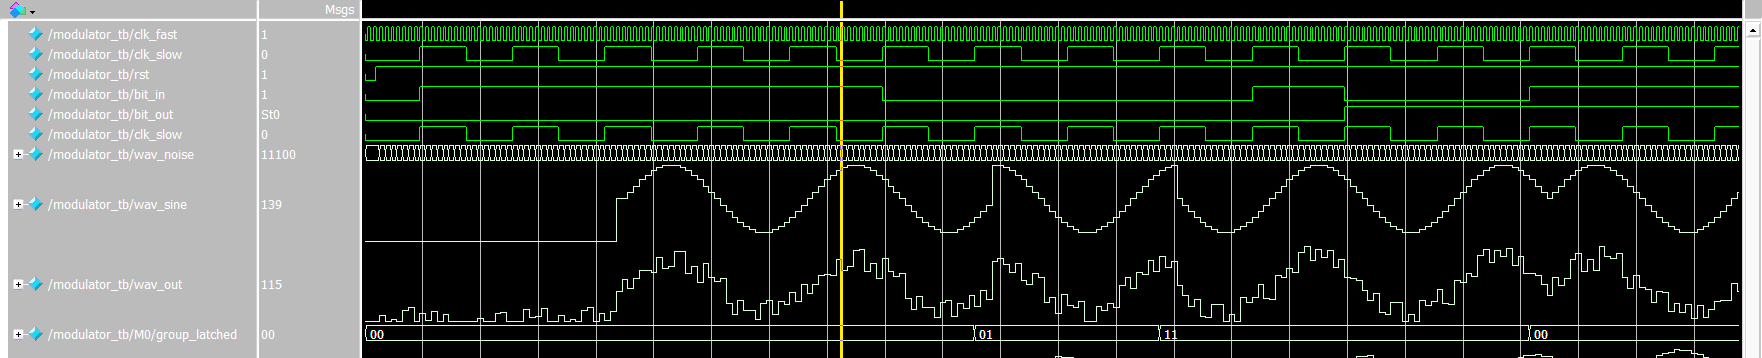
\includegraphics[width = .9\textwidth]{images//modulator_out.png}\vspace{10pt}\par
使用5bit的移位寄存器完成附加帧头的功能。可以观察到,初始波形输出的确是相移为0正弦信号的2个完整周期。随后$b_0b_1$数据存到\texttt{group\_latched[1:0]} 中,生成不同相位的正弦波形。附加起始帧头导致\texttt{group\_latched[1:0]} 中的数据是5--6 个慢时钟周期之前的输入比特流\texttt{bit\_in}。\par\par

对于\textbf{信道加噪模块}(详细代码见\texttt{modulation/pseudo\_random.v},我们从网上找到了一个伪随机数发生器实现,并加入到系统实现中。伪随机数发生器模块输出位宽是5bit,使用原码,最高位是符号位。输出乘以2后和调制输出数据\texttt{wav\_out[7:0]} 相加。如果结果小于0,则相加结果置为0;如果结果大于8bit表示最大值,结果直接置为255。于是噪声信号的最大值是有用信号最大值的1/8。正弦波信号和加入噪声后信号的仿真波形如下:\par
\vspace{10pt}
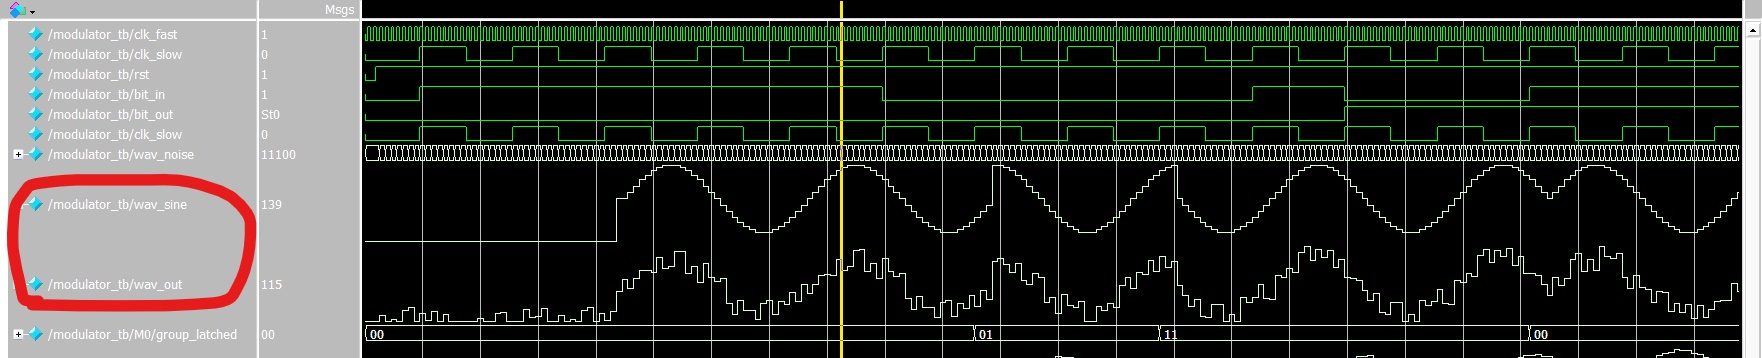
\includegraphics[width = .9\textwidth]{images//noise_addition.jpg}\vspace{10pt}\par

对于\textbf{解调模块}(详细代码见\texttt{modulation/demodulator.v}),输入输出为
\begin{itemize}
\item \texttt{input clk\_fast, clk\_slow, rst; input [7:0] wav\_in;}
\item \texttt{output reg bit\_out; output valid;}
\end{itemize}
功能可以分成两部分:帧头同步和符号判决。两个部分核心都是相关运算。相关运算单元由32个乘法器和5 级加法树组成,有6个快时钟周期的延迟。解调模块会使用移位寄存器保存32个周期的输入数据,用来和零相位正弦波/余弦波做相关。因此,当输入信号也是一个零相移的正弦波信号时,正弦波相关结果是一个峰值。每个快时钟周期,相关运算结果都会更新。\par

输入只是噪声时,这些相关结果近似为0。当有用信号开始输入时,因为帧头的存在,最开始的有效波形一定是2个慢时钟周期的零相位偏移正弦波+ 噪声,显示在相关的输出上就是两个与正弦波做相关的峰。帧头同步的功能就是捕捉这些峰值的时刻。为了排除其他值较小的峰值影响,定义一个\texttt{HIGH\_TH},只有相关结果大于这个门限值时,我们才捕捉峰值的存在。为简单起见,我们只捕捉输入第一个帧头对应正弦波的相关峰。一旦捕捉到一个大于\texttt{HIGH\_TH} 的相关峰,相位匹配就完成了,因为我们知道了第一个符号对应波形的起始时刻,就可以推测之后任意一个符号波形的起始时刻。峰值的捕捉由一个简单的状态机完成。\par

完成同步后,系统跳过第二个相关峰(仍由帧头数据产生),进行真实数据符号的判决。每两个慢时钟周期,系统会读取正弦波相关数据和余弦波相关数据。可以把它们分别记作$R_{sin}, R_{cos}$,根据表格2定义的规则进行符号判决。实际系统中HIGH, LOW门限的值分别为\texttt{200000, 120000}。仿真结果如下:\par
\vspace{10pt}
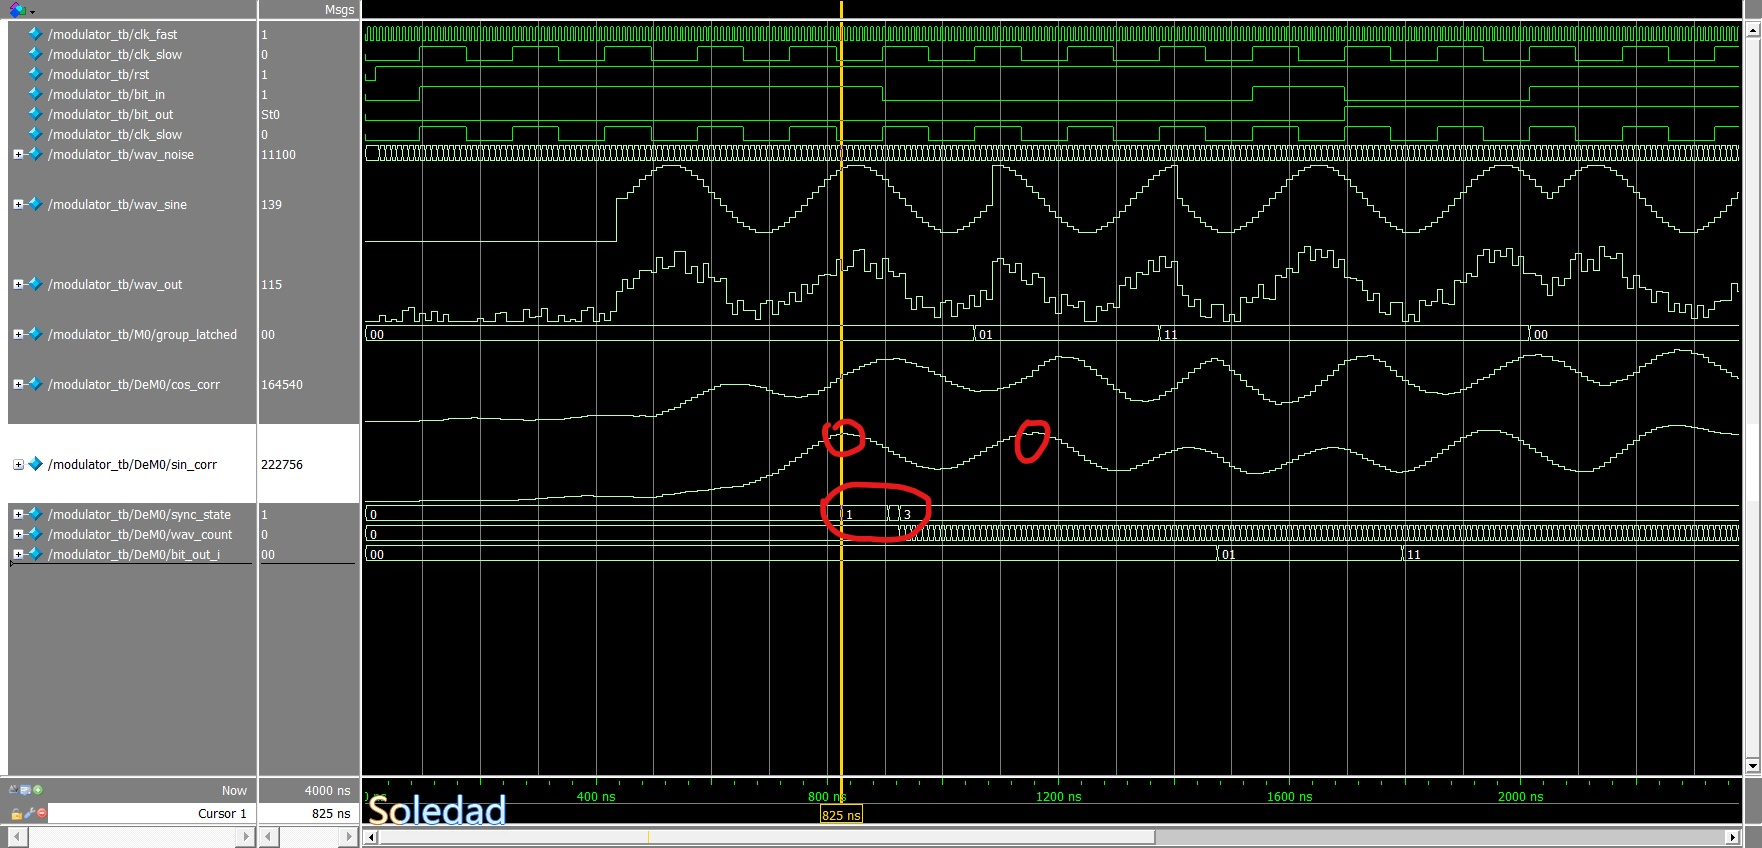
\includegraphics[width = .9\textwidth]{images//demodulator.jpg}\vspace{10pt}\par
帧头带来的两个相关峰被圈注出来了。下方用红笔圈注表示用于捕捉峰值状态机状态的变化,第一个峰值被捕捉后,状态就不再改变。最下方的\texttt{bit\_out\_i[1:0]}是判决的符号结果,可以和\texttt{group\_latched[1:0]}做对比。除了有约2个慢时钟周期的延迟外,数据没有出错,而且解调输出中没有帧头数据。\par

下图是略去中间实现细节,整个调制解调系统的输入输出仿真结果:\par
\vspace{10pt}
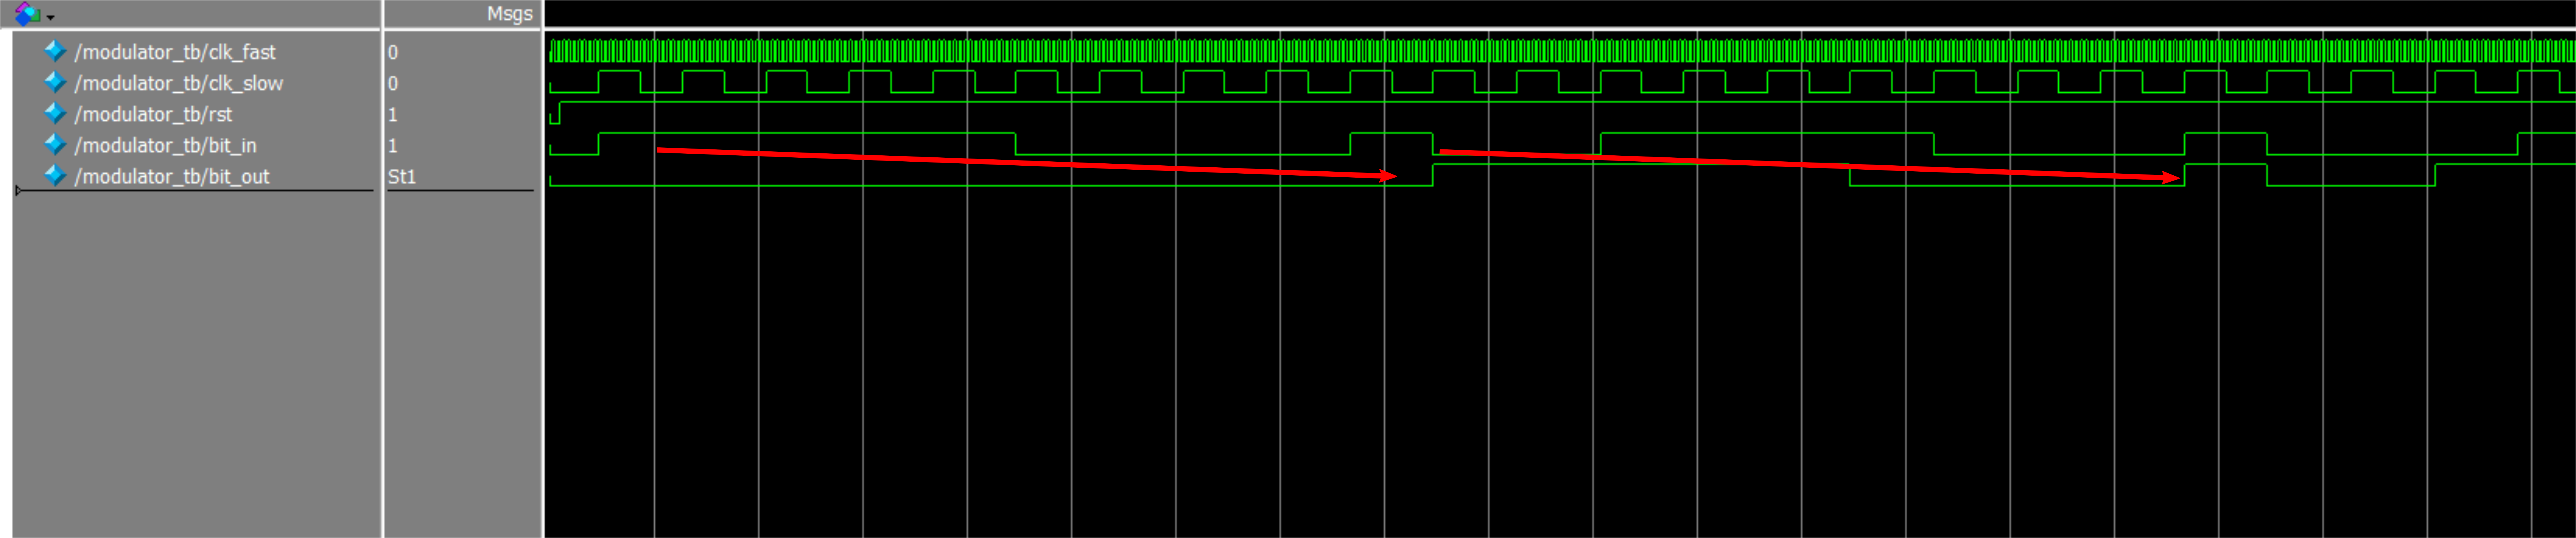
\includegraphics[width = .9\textwidth]{images//mod_demod.png}\vspace{10pt}\par
红色箭头标示了输入输出信号的延迟。